\documentclass[12pt,a4paper]{report}
\usepackage[a4paper,margin=1in]{geometry}
\usepackage[T1]{fontenc}
\usepackage[utf8]{inputenc}
\usepackage{lmodern}
\usepackage{microtype}
\usepackage{graphicx}
\usepackage{booktabs}
\usepackage{longtable}
\usepackage{array}
\usepackage{tabularx}
\usepackage{enumitem}
\usepackage{float}
\usepackage{caption}
\usepackage{subcaption}
\usepackage{hyperref}
\usepackage{xcolor}
\usepackage{listings}
\usepackage{fancyhdr}
\usepackage{titlesec}
\usepackage{tikz}
\usepackage{placeins}
\usepackage{amsmath}
\usepackage{url}
\usepackage{lastpage}
\hypersetup{colorlinks=true,linkcolor=blue!55!black,urlcolor=blue!55!black,citecolor=blue!55!black,pdftitle={IntrudeAware - Intelligent Video Surveillance and Scene Analysis},pdfauthor={Shlok Khanna}}
\definecolor{codebg}{RGB}{248,250,252}
\definecolor{codeborder}{RGB}{203,213,225}
\definecolor{codekw}{RGB}{30,64,175}
\definecolor{codecomment}{RGB}{71,85,105}
\lstset{backgroundcolor=\color{codebg},frame=single,rulecolor=\color{codeborder},basicstyle=\ttfamily\small,keywordstyle=\color{codekw}\bfseries,commentstyle=\color{codecomment}\itshape,showstringspaces=false,breaklines=true,columns=fullflexible}
\pagestyle{fancy}
\fancyhf{}
\setlength{\headheight}{15pt}
\lhead{IntrudeAware}
\rhead{CSE3010 Computer Vision}
\cfoot{Page \thepage}
\titleformat{\chapter}[display]{\bfseries\Huge}{\chaptertitlename\ \thechapter}{12pt}{\Huge}
\setlength{\parindent}{0pt}
\setlength{\parskip}{6pt}
\newcommand{\projectname}{IntrudeAware}
\newcommand{\code}[1]{\texttt{#1}}

\begin{document}

\begin{titlepage}
\centering
\vspace*{1.0cm}
{\Large \textbf{CSE3010 - COMPUTER VISION}}\\[0.6cm]
{\Huge \textbf{IntrudeAware}}\\[0.25cm]
{\LARGE Intelligent Video Surveillance and Scene Analysis}\\[0.6cm]
{\large Adaptive YOLO Detection, Multi-Object Tracking, Motion Analysis and Restricted-Zone Events}\\[1.0cm]
\rule{0.82\textwidth}{0.8pt}\\[0.8cm]
\begin{tabular}{>{\bfseries}p{0.30\textwidth}p{0.50\textwidth}}
Student Name & Shlok Khanna \\
Registration No. & 24BAI10235 \\
Program  & B.Tech. CSE-AIML \\
Course & CSE3010 Computer Vision \\
Project Type & VITyarthi \\
Academic Year & 2026 \\
\end{tabular}
\vfill
{\large Final Submission Package}\par
\vspace{0.4cm}
{\small Prepared as an academic prototype aligned with the supplied CSE3010 syllabus and VITyarthi project guidelines.}
\end{titlepage}

\pagenumbering{roman}
\chapter*{Abstract}
\addcontentsline{toc}{chapter}{Abstract}
\projectname{} is a modular computer-vision application that transforms uploaded video into semantic detections, persistent object tracks, motion measurements, restricted-zone state transitions, and visual analytics. The system combines image preprocessing, Ultralytics YOLO semantic detection, a persistent centroid tracker, sparse Lucas-Kanade optical flow, rule-based zone-event detection, and a Streamlit dashboard. The design keeps the tracker and event engine independent of the detector, allowing the semantic detector to be refreshed less frequently than the video frame rate. An adaptive scheduling policy uses smoothed object velocity and restricted-zone activity to request more frequent YOLO inference during meaningful motion while reducing unnecessary inference in calmer scenes. A short refresh cooldown is added to reduce scheduler oscillation caused by noisy frame-to-frame motion.

The project is intentionally modular and explainable. It includes automated tests, configurable CPU/CUDA inference, browser-compatible video output, timestamped ENTRY/EXIT events, CSV export, design diagrams, and an evaluation plan. The implementation aligns with the course emphasis on image preprocessing, motion analysis, object detection/tracking, and development of computer-vision applications. The final report separates measured project results from external vendor benchmarks and includes a reproducible evaluation protocol rather than inventing unmeasured performance values.

\textbf{Keywords:} computer vision, YOLO, object detection, object tracking, optical flow, restricted-zone detection, adaptive inference, Streamlit.

\tableofcontents
\listoffigures
\listoftables
\clearpage
\pagenumbering{arabic}

\chapter{Introduction}
The supplied CSE3010 syllabus states that the course covers the theoretical and practical aspects of computing with images, image formation and analysis, major computer-vision methods, and the development of computer-vision applications \cite{cse3010_syllabus}. Its indicative practical work includes image preprocessing and edge detection, segmentation, optical flow, object detection and tracking from video, dynamic-background surveillance, and related 3D-vision tasks. IntrudeAware was designed to combine several of these concepts into one coherent application rather than implementing isolated laboratory exercises.

The VITyarthi guide requires an original project aligned with the subject, at least three major functional modules, clear input/output, a logical workflow, non-functional requirements, modular implementation, testing, design artifacts, and a final report \cite{vityarthi_guide}. IntrudeAware therefore treats the video-analysis pipeline, event engine, dashboard, and adaptive inference scheduler as one integrated system.

\section{Project Motivation}
Continuous video contains a large number of frames, while the semantic content of the scene often changes more slowly than the raw frame rate. Running a semantic detector on every frame can therefore be computationally expensive. At the same time, zone-entry events and object motion require timely updates. The project addresses this tension by separating semantic detection from the downstream tracking and event layers.

\section{Project Goals}
\begin{enumerate}[leftmargin=*]
  \item Build a usable computer-vision application for uploaded video.
  \item Demonstrate CSE3010 concepts through an integrated pipeline.
  \item Preserve persistent track IDs between semantic detector refreshes.
  \item Produce interpretable restricted-zone ENTRY/EXIT events with timestamps.
  \item Reduce unnecessary YOLO inference with adaptive scheduling while retaining frame-level visualization and event updates.
  \item Provide a reproducible evaluation and documentation package.
\end{enumerate}

\chapter{Problem Statement, Scope and Objectives}
\section{Problem Statement}
Manual monitoring of continuous video is repetitive and makes it difficult to consistently record object movement and zone events. IntrudeAware processes an uploaded video, detects supported semantic object classes, assigns persistent track IDs, estimates motion, monitors a user-defined restricted region, and presents the results as an annotated video and event dashboard.

\section{Scope}
The final project focuses on uploaded video files. The system performs:
\begin{itemize}[leftmargin=*]
  \item frame preprocessing and enhancement;
  \item YOLO-based semantic detection;
  \item multi-object tracking with persistent IDs and intermediate-frame prediction;
  \item sparse optical-flow analysis;
  \item restricted-zone ENTRY/EXIT event detection;
  \item adaptive YOLO frame scheduling with velocity smoothing and a cooldown;
  \item interactive visualization and CSV event export.
\end{itemize}
The project is an academic prototype and is not presented as a safety-critical surveillance product.

\section{Objectives}
\begin{enumerate}[leftmargin=*]
  \item Implement an end-to-end computer-vision video pipeline.
  \item Demonstrate preprocessing, filtering, edge detection, motion computation, object detection, tracking, and event analysis.
  \item Maintain stable object identities across detector refreshes.
  \item Generate non-duplicated zone entry events and explicit exit events.
  \item Compare inference scheduling strategies using reproducible measurements.
  \item Deliver modular source code and formal design documentation.
\end{enumerate}

\chapter{Requirements Analysis}
\section{Functional Requirements}
\begin{enumerate}[leftmargin=*]
  \item The system shall accept MP4, AVI, MOV, and MKV video files.
  \item The system shall preprocess video frames using resizing, Gaussian filtering, contrast enhancement, and Canny edge detection.
  \item The system shall run YOLO semantic detection on supported classes and expose model size, confidence, and device controls.
  \item The system shall maintain persistent track IDs across detection refreshes.
  \item The system shall continue to update track positions on intermediate frames using the existing tracker prediction logic.
  \item The system shall monitor a rectangular restricted zone.
  \item The system shall generate ENTRY and EXIT events when a track changes zone state.
  \item The system shall retain zone state during short detection gaps to avoid duplicate entries.
  \item The system shall show track IDs, semantic labels, and IN ZONE status on the output frame.
  \item The system shall show dashboard metrics and provide event CSV export.
\end{enumerate}

\section{Non-Functional Requirements}
\begin{longtable}{>{\bfseries}p{0.22\textwidth}p{0.68\textwidth}}
\toprule
Requirement & Description\\
\midrule
Performance & Adaptive scheduling should reduce unnecessary YOLO calls while preserving frame-level tracker, event, and overlay updates.\\
Usability & All major settings shall be available from the Streamlit sidebar.\\
Reliability & Invalid inputs and detector failures should not silently corrupt event state.\\
Maintainability & Detector, tracker, motion, event, visualization, and UI components are separated into modules.\\
Scalability & The semantic detector can be changed without redesigning the event and visualization layers.\\
Logging & Processing and event information can be inspected through the dashboard and CSV export.\\
Resource efficiency & Model scale, device, frame skipping, smoothing, and cooldown are configurable.\\
\bottomrule
\end{longtable}

\section{Target Users}
The primary users are computer-vision students, academic demonstrators, researchers prototyping video-analysis pipelines, and developers learning applied computer vision.

\chapter{System Architecture and Design}
\section{High-Level Architecture}
Figure~\ref{fig:architecture} shows the separation between video input, preprocessing, semantic detection, tracking, motion analysis, event analysis, visualization, and reporting.
\begin{figure}[H]\centering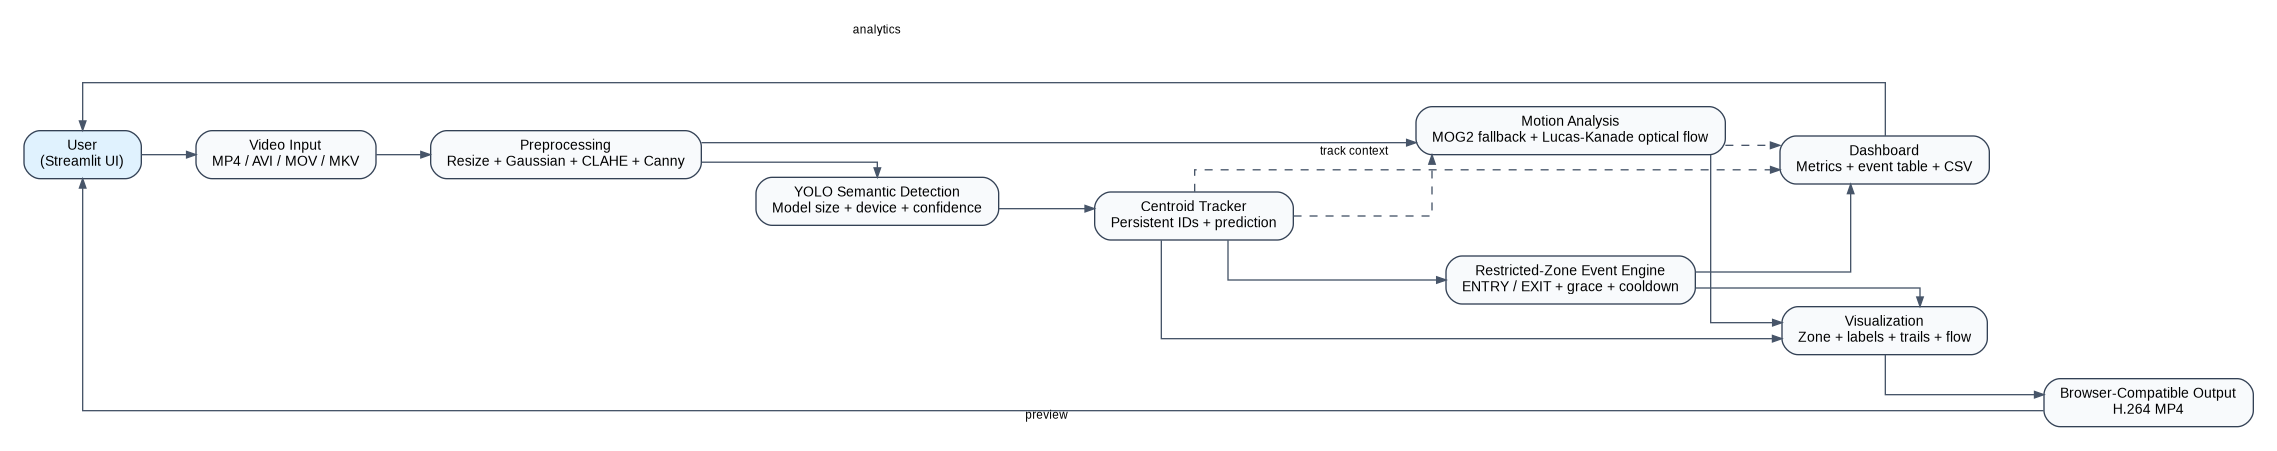
\includegraphics[width=\textwidth]{diagrams/architecture.png}\caption{IntrudeAware system architecture.}\label{fig:architecture}\end{figure}

\section{Process Workflow}
The workflow is frame-oriented. YOLO may refresh only when the adaptive scheduler requests it. Intermediate frames are still passed through tracker prediction, optical-flow computation, zone state updates, overlay generation, and output writing.
\begin{figure}[H]\centering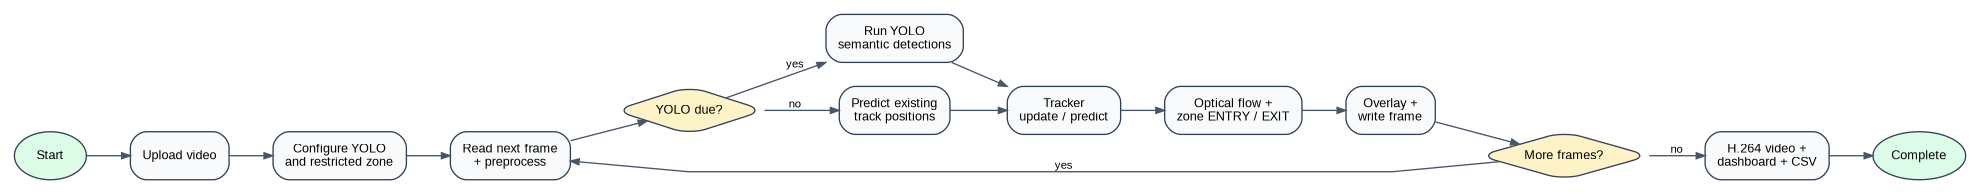
\includegraphics[width=\textwidth]{diagrams/workflow.png}\caption{IntrudeAware processing workflow.}\label{fig:workflow}\end{figure}

\section{Use Case Diagram}
\begin{figure}[H]\centering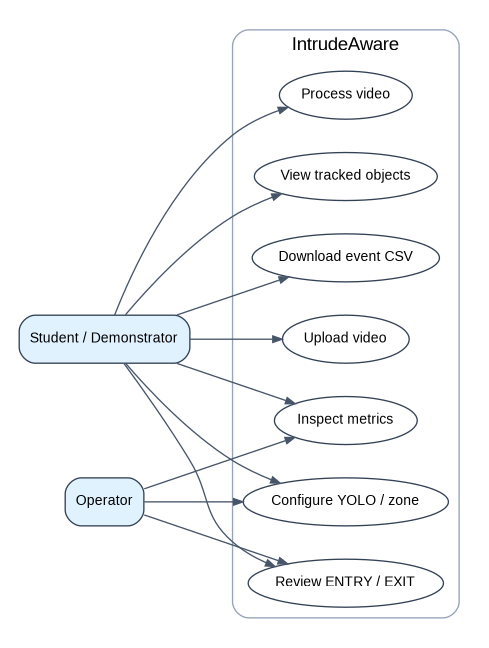
\includegraphics[width=0.92\textwidth]{diagrams/use_case.png}\caption{Use case diagram.}\label{fig:usecase}\end{figure}

\section{Sequence Diagram}
\begin{figure}[H]\centering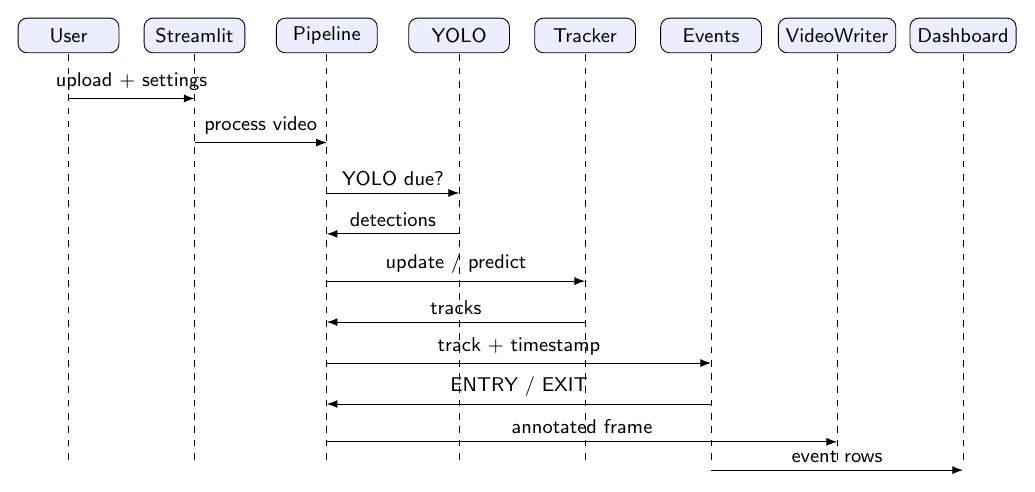
\includegraphics[width=\textwidth]{diagrams/sequence.png}\caption{Sequence-oriented interaction diagram for one video-processing session.}\label{fig:sequence}\end{figure}

\section{Class and Component View}
\begin{figure}[H]\centering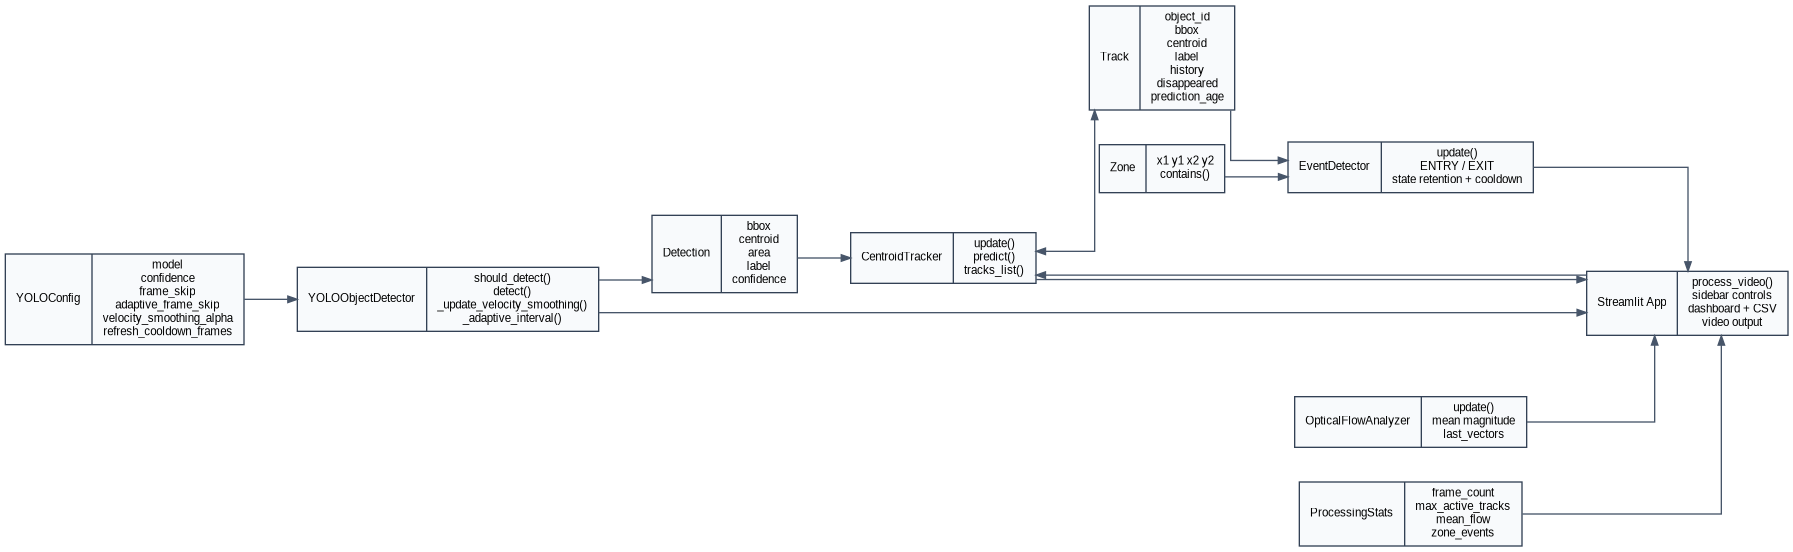
\includegraphics[width=\textwidth]{diagrams/class.png}\caption{Class/component relationships used by the project.}\label{fig:class}\end{figure}

\section{Design Decisions}
\begin{itemize}[leftmargin=*]
  \item \textbf{Detector abstraction:} YOLO detections are converted into the existing \code{Detection} structure, so the tracker and event engine do not depend on Ultralytics internals.
  \item \textbf{Persistent tracking:} the existing centroid tracker remains responsible for track IDs, not the semantic detector.
  \item \textbf{Event state retention:} zone state is retained through short missing periods to prevent duplicate ENTRY events caused by temporary detector loss.
  \item \textbf{Adaptive scheduling:} semantic inference frequency is controlled separately from the output frame rate.
  \item \textbf{Configuration:} model, device, confidence, frame skip, smoothing, cooldown, and zone geometry are exposed as parameters.
\end{itemize}

\chapter{Computer Vision Methodology}
\section{Image Preprocessing}
Each frame is resized to a working width, converted for processing, smoothed with a Gaussian kernel, enhanced with CLAHE, and optionally converted to an edge map using Canny. These operations correspond to the low-level image-processing concepts emphasized in the course syllabus \cite{cse3010_syllabus}.

\section{Semantic Object Detection with YOLO}
IntrudeAware uses a pretrained Ultralytics YOLO26 detector. The application currently exposes the nano, small, medium, large, and extra-large detection scales and passes the selected device explicitly to the detector. Ultralytics documents the YOLO26 family, the five detection scales, and Python inference through the \code{YOLO()} interface \cite{ultralytics_yolo26}.

The project maps the model's COCO class names to a small application vocabulary:
\begin{center}
\begin{tabular}{ll}
\toprule
YOLO class & IntrudeAware label\\
\midrule
person & PERSON\\
bicycle & BIKE\\
motorcycle & BIKE\\
car & CAR\\
bus & BUS\\
truck & TRUCK\\
\bottomrule
\end{tabular}
\end{center}
Unsupported classes are ignored by the application layer.

\subsection{Model-size rationale}
The project defaults to YOLO26n because the smallest model provides a practical baseline for an academic laptop while preserving the same API shape used by larger variants. Ultralytics publishes model-family benchmark figures for its own reference environments; these values are not treated as IntrudeAware performance measurements \cite{ultralytics_yolo26}. The final project evaluation must use the actual target machine and fixed evaluation video.

\section{Object Tracking}
The tracker associates detections to existing tracks using nearest-centroid matching subject to a configurable maximum distance. Every track stores an object ID, bounding box, centroid, label, trajectory history, disappearance count, and prediction age.

When YOLO is skipped on an intermediate frame, the tracker estimates the next centroid from the last two trajectory points. This preserves visualization continuity and supplies a predicted state to the event detector.

\section{Optical Flow}
Sparse Lucas-Kanade optical flow estimates local point motion between consecutive preprocessed frames. The system records flow vectors and computes a mean magnitude used in the dashboard and as contextual motion evidence.

\section{Restricted-Zone Event Detection}
A zone is represented by a rectangular region in frame coordinates. A track generates an ENTRY when it transitions from outside to inside and an EXIT when it transitions from inside to outside. Two safeguards reduce duplicate events: a missing-frame grace period and a re-entry cooldown.

\section{Adaptive YOLO Frame Scheduling}
Let $v_t$ be the maximum observed track speed in pixels per frame at time $t$. The scheduler maintains an exponentially weighted moving average:
\[
\hat{v}_t = \alpha v_t + (1-\alpha)\hat{v}_{t-1}, \qquad 0 < \alpha \le 1.
\]
The desired detector interval is then selected from three levels: the configured maximum interval for calm motion, a shorter interval for moderate motion, and one-frame refresh for fast motion or an active in-zone track. A minimum refresh cooldown is applied after the desired interval is selected.

This separates semantic inference frequency from the output frame rate: all frames continue through tracking, event analysis, visualization, and video writing even when YOLO is not invoked.

\chapter{Software Implementation}
\section{Technology Stack}
\begin{center}
\begin{tabular}{ll}
\toprule
Layer & Technology\\
\midrule
Language & Python\\
Image processing & OpenCV\\
Numerical operations & NumPy\\
Semantic detection & Ultralytics YOLO26\\
Data handling & Pandas\\
Dashboard & Streamlit\\
Video encoding helper & imageio-ffmpeg\\
Testing & Pytest\\
Version control & Git / GitHub\\
\bottomrule
\end{tabular}
\end{center}

\section{Repository Structure}
The repository is divided by responsibility so that changes to the semantic detector do not force changes to the tracker, event logic, or dashboard. The source tree includes the preprocessing, detection, tracking, motion, analysis, visualization, utility, configuration, evaluation, and test modules.

\section{Important Modules}
\begin{longtable}{>{\raggedright\arraybackslash}p{0.34\textwidth}p{0.54\textwidth}}
\toprule
Module & Role\\
\midrule
\path{app.py} & Streamlit interface and end-to-end video processing loop.\\
\path{detection/yolo_detector.py} & YOLO loading, semantic filtering, adaptive scheduling, velocity smoothing, and cooldown.\\
\path{tracking/tracker.py} & Persistent centroid tracks and intermediate-frame prediction.\\
\path{analysis/event_detection.py} & Zone state machine and timestamped ENTRY/EXIT events.\\
\path{motion/optical_flow.py} & Sparse Lucas-Kanade motion analysis.\\
\path{visualization/drawing.py} & Restricted-zone overlay, labels, trails, and frame metrics.\\
\path{analysis/statistics.py} & Processing statistics.\\
\bottomrule
\end{longtable}

\section{Representative Scheduling Code}
\begin{lstlisting}[language=Python,caption={Adaptive scheduling rule used by YOLOObjectDetector}]
smoothed_speed = self._update_velocity_smoothing(tracks)

any_inside = any(
    track.disappeared == 0 and _inside_zone(track, zone_bounds)
    for track in tracks
)

if any_inside:
    return 1
if smoothed_speed >= self.cfg.high_speed_px_per_frame:
    return 1
if smoothed_speed >= self.cfg.medium_speed_px_per_frame:
    return min(2, self.cfg.frame_skip)
return self.cfg.frame_skip
\end{lstlisting}

\chapter{User Interface and Results Visualization}
\section{Dashboard}
The Streamlit dashboard provides controls for model size, device, confidence threshold, maximum frame skip, adaptive scheduling, velocity smoothing, refresh cooldown, optical-flow vectors, Canny overlay, and restricted-zone geometry.

\begin{figure}[H]\centering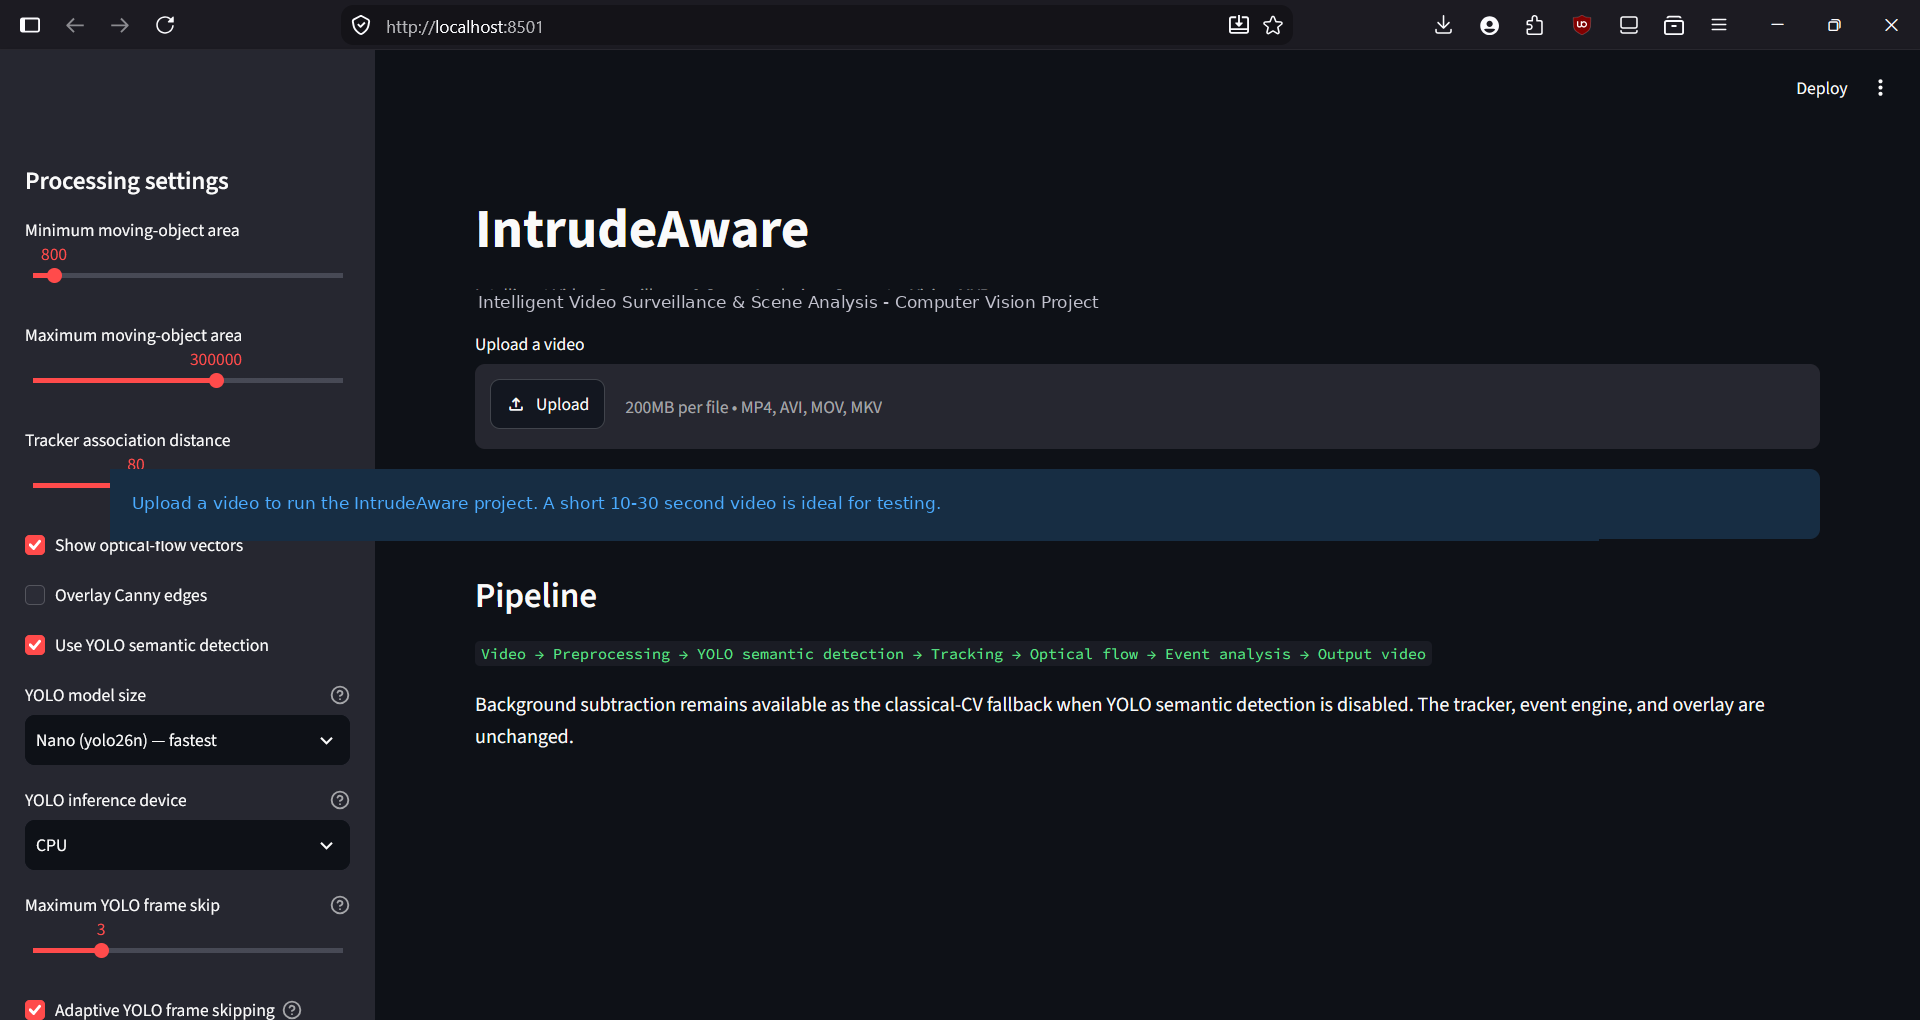
\includegraphics[width=\textwidth]{figures/dashboard_settings.png}\caption{IntrudeAware dashboard at runtime with upload, motion, YOLO, and restricted-zone controls.}\label{fig:dashboard}\end{figure}

\section{Video Overlay}
The processed video highlights the restricted zone, labels every active track with an ID and semantic class, and appends \code{IN ZONE} for tracks currently inside the protected region.

\begin{figure}[H]\centering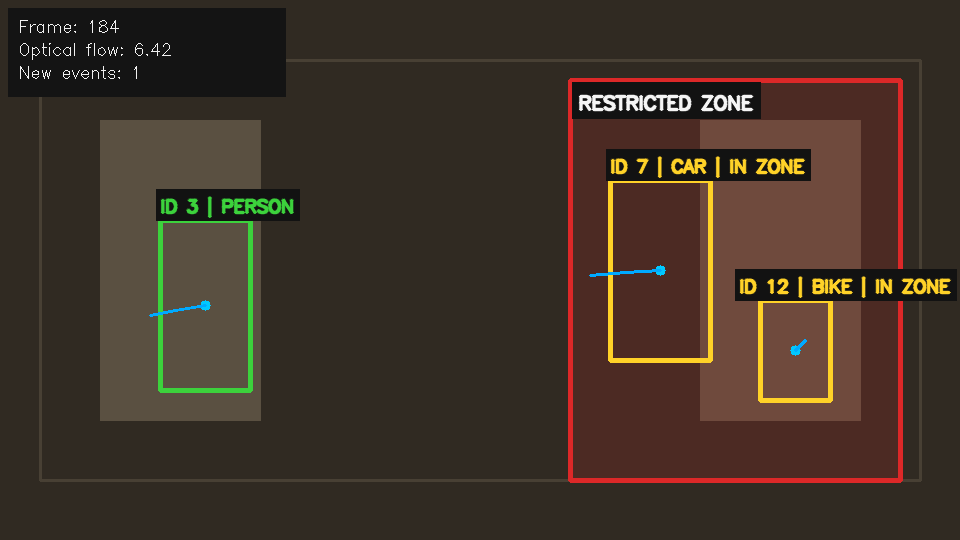
\includegraphics[width=0.94\textwidth]{figures/overlay_example.png}\caption{Illustrative IntrudeAware output overlay generated from the project drawing functions.}\label{fig:overlay}\end{figure}

\section{Event Dashboard}
Each event row contains the relative video timestamp, frame number, track ID, ENTRY/EXIT status, and a human-readable message. The table can be filtered by event status and downloaded as CSV. The relative timestamp is computed as frame index divided by the video FPS, so it remains tied to the analyzed video rather than the system clock.

\section{Final Runtime Configuration and Runtime Evidence}
The final settings view supplied with the project records the processing thresholds and the YOLO/adaptive-inference configuration used for the run.

\begin{figure}[H]
\centering
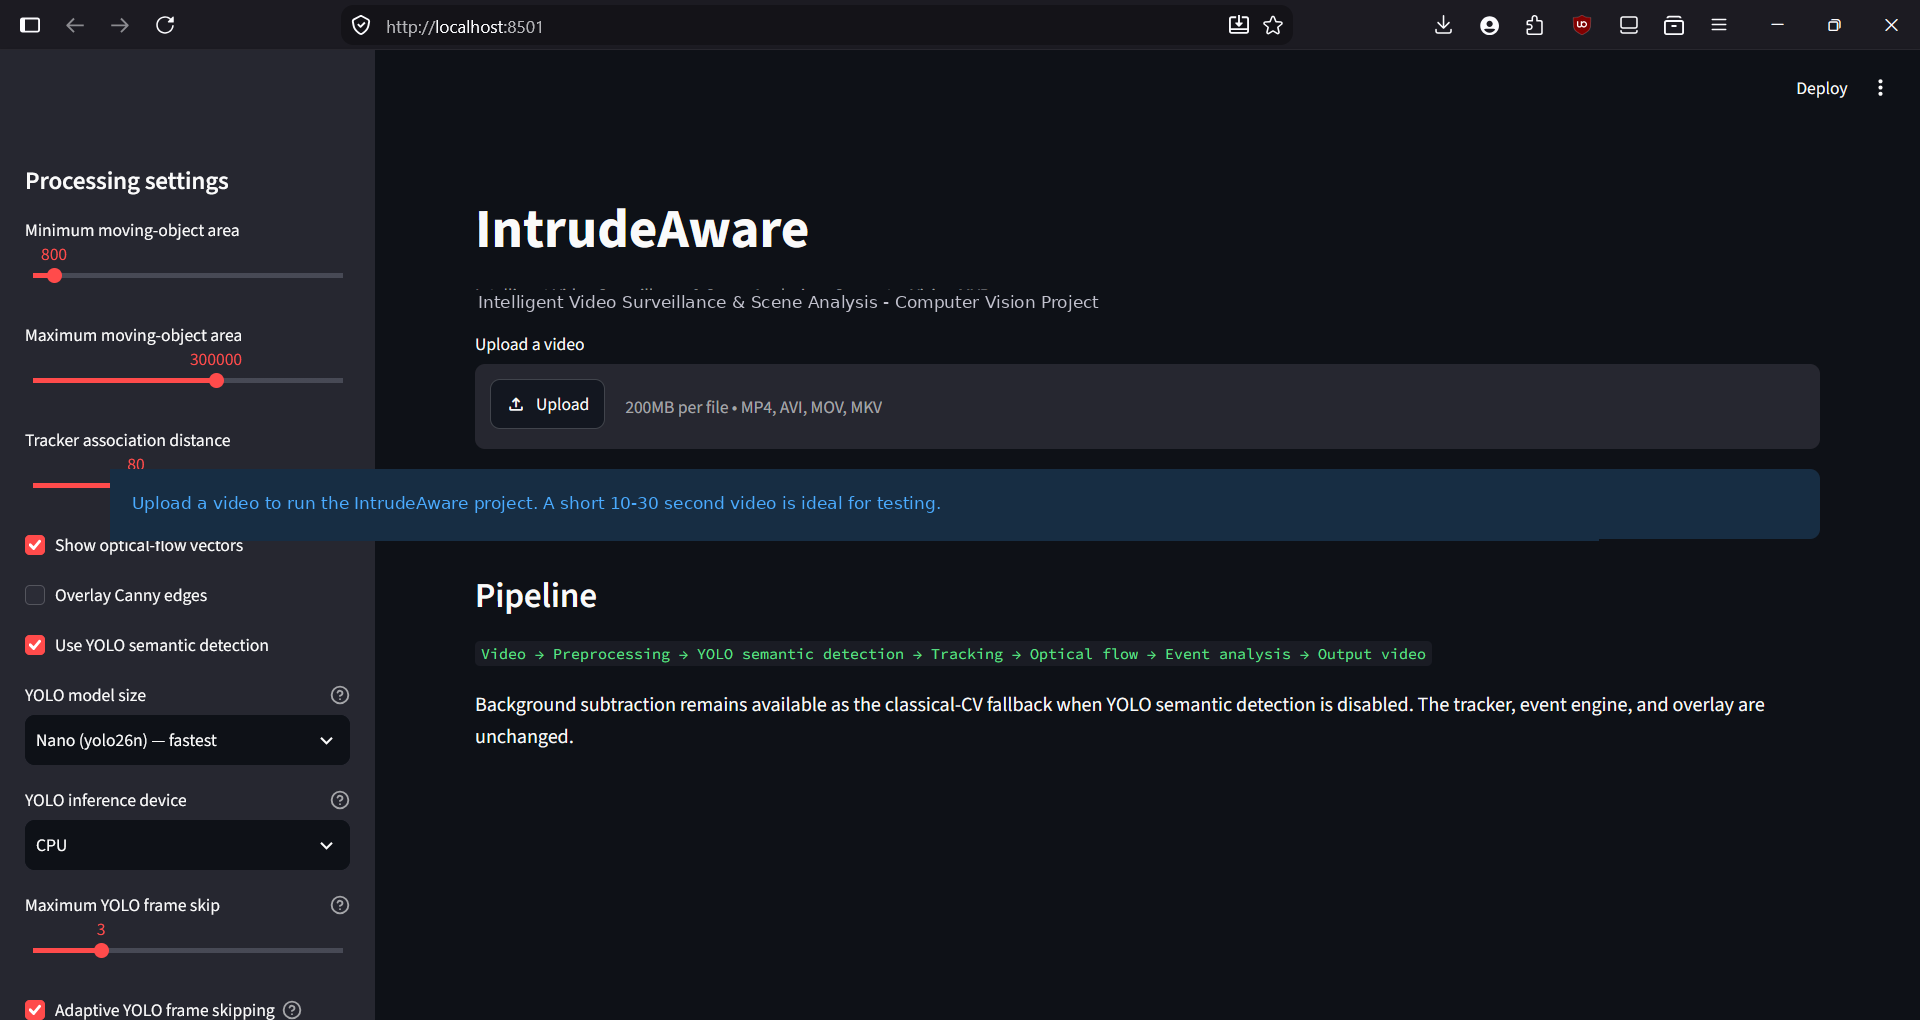
\includegraphics[width=\textwidth]{figures/dashboard_settings.png}
\caption{IntrudeAware dashboard showing the final project settings before processing, including YOLO26n, CPU inference, frame skipping, and adaptive scheduling.}
\label{fig:settings}
\end{figure}


The supplied runtime screenshots document the final IntrudeAware configuration and its observable outputs. The processed-video view shows persistent track IDs, semantic labels, the highlighted restricted zone, optical-flow information, and in-zone status. The event-dashboard screenshots show timestamped ENTRY/EXIT rows, track IDs, event messages, and the processing summary.

\begin{figure}[H]
\centering
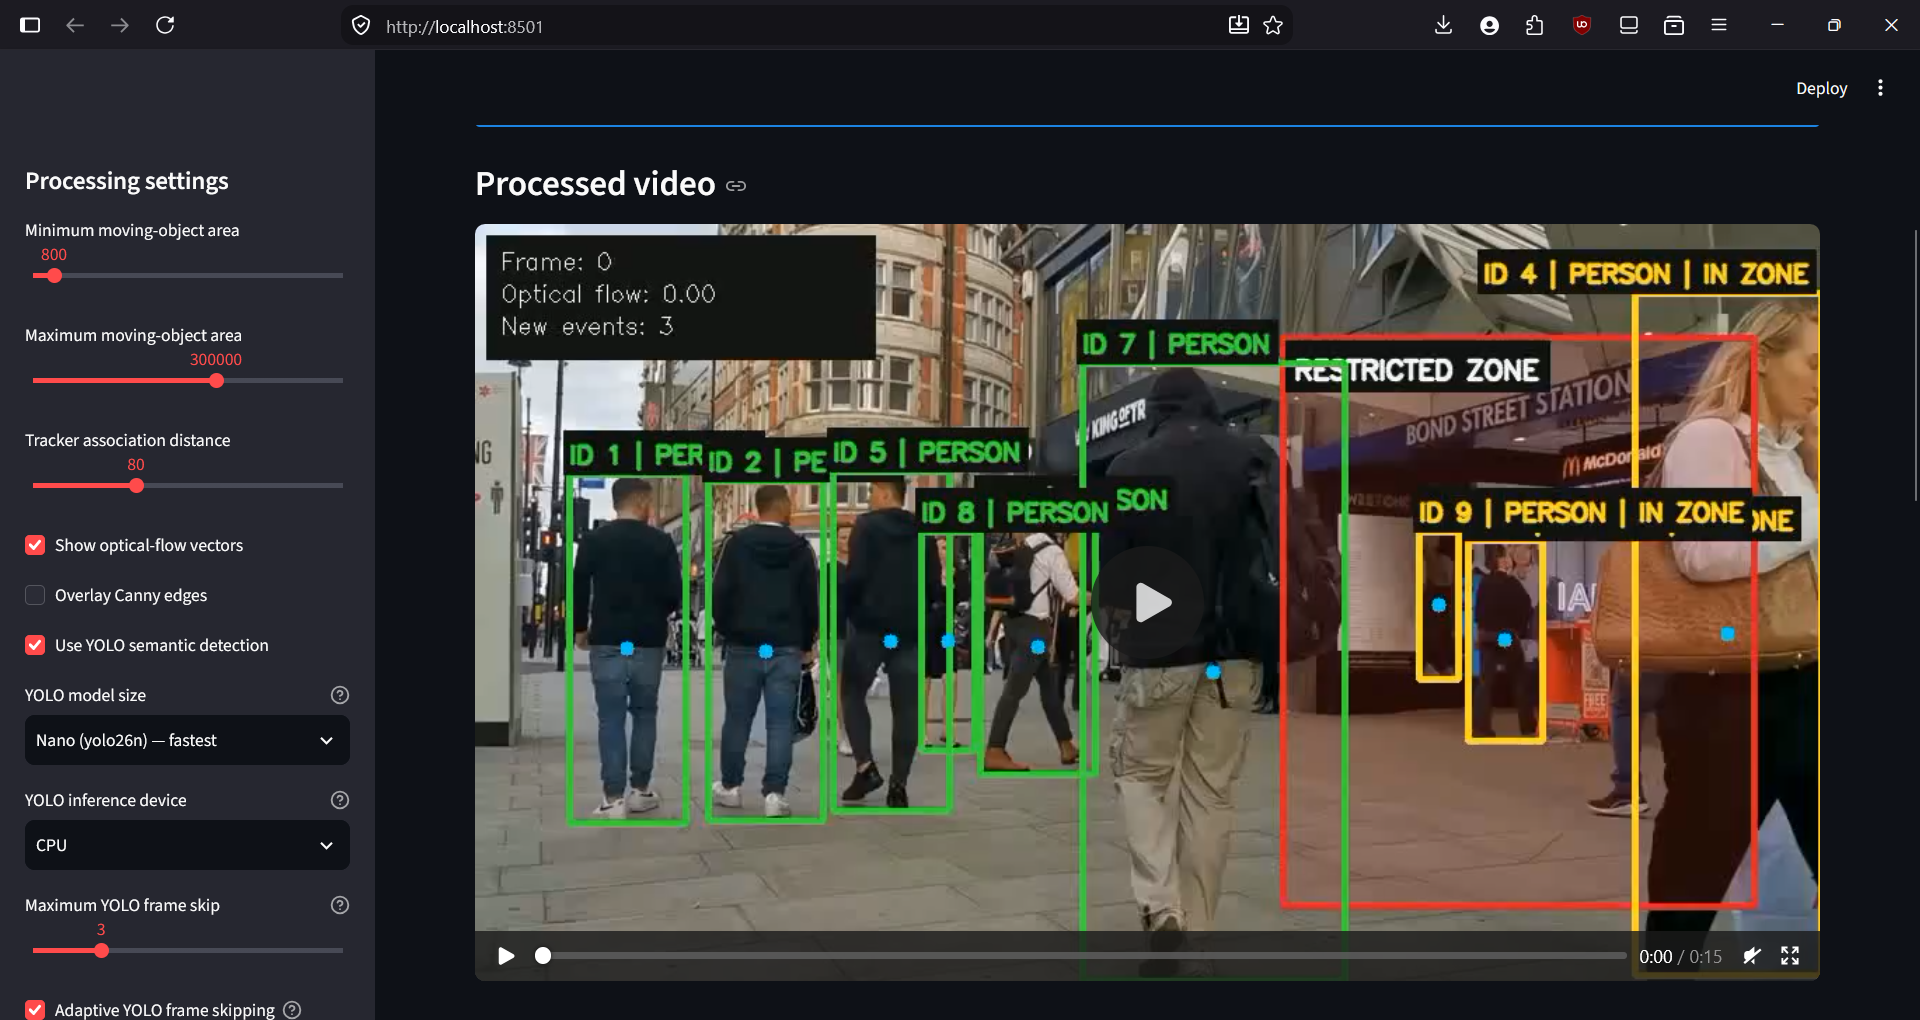
\includegraphics[width=\textwidth]{figures/dashboard_overlay.png}
\caption{IntrudeAware processed-video view showing semantic labels, persistent track IDs, restricted-zone highlighting, and in-zone status.}
\label{fig:runtime_overlay}
\end{figure}

\begin{figure}[H]
\centering
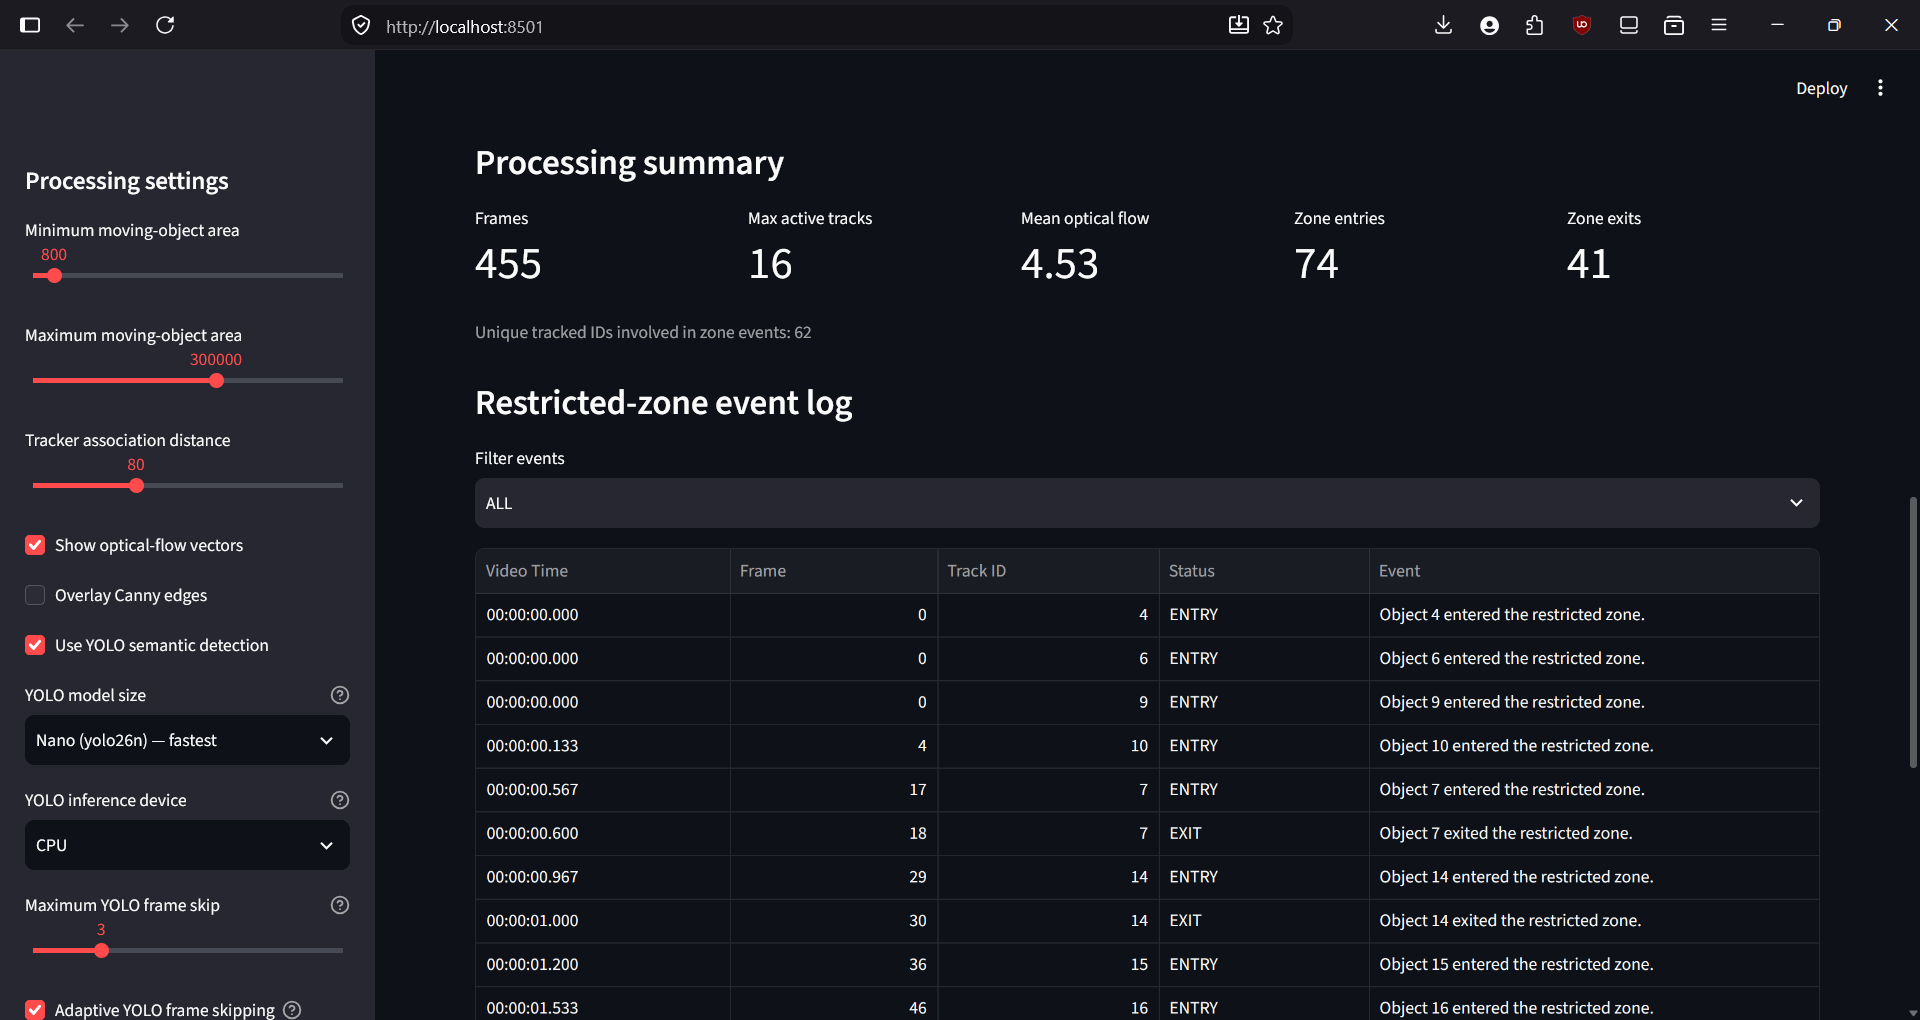
\includegraphics[width=\textwidth]{figures/event_dashboard.png}
\caption{IntrudeAware processing summary and restricted-zone event dashboard.}
\label{fig:event_dashboard}
\end{figure}

\begin{figure}[H]
\centering
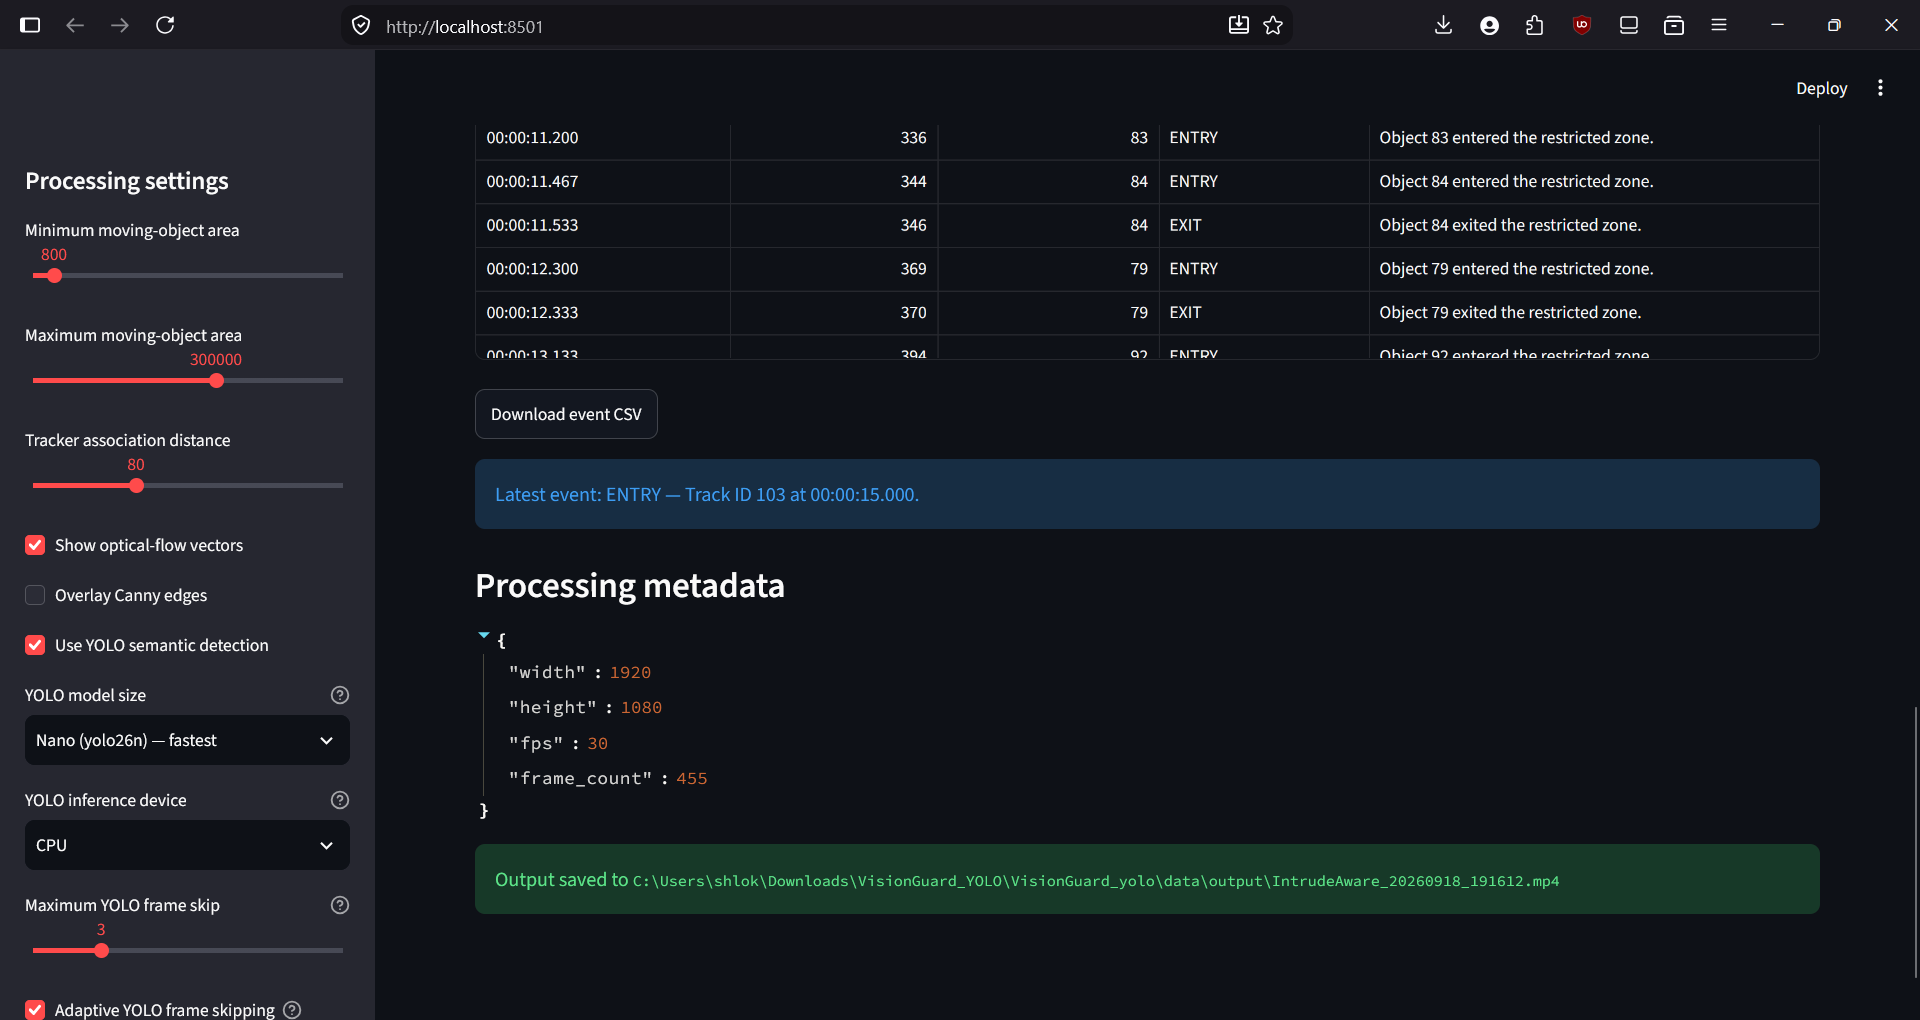
\includegraphics[width=\textwidth]{figures/event_metadata.png}
\caption{IntrudeAware event-log tail, latest event, processing metadata, and saved output path.}
\label{fig:event_metadata}
\end{figure}

\begin{table}[H]
\centering
\caption{Visible runtime settings recorded in the supplied screenshots.}
\label{tab:runtime_settings}
\begin{tabular}{ll}
\toprule
Setting & Observed value\\
\midrule
Minimum moving-object area & 800\\
Maximum moving-object area & 300000\\
Tracker association distance & 80\\
Optical-flow vectors & Enabled\\
Canny overlay & Disabled\\
YOLO semantic detection & Enabled\\
YOLO model & Nano (\code{yolo26n})\\
Inference device & CPU\\
Maximum YOLO frame skip & 3\\
Adaptive YOLO frame skipping & Enabled\\
\bottomrule
\end{tabular}
\end{table}

\section{Observed Event-Log Evidence}
A runtime event CSV was also captured from the processed video and included in the submission package as \code{report/evidence/intrudeaware\_events.csv}. The supplied log contains 115 recorded events across 62 unique track IDs, covering video-relative timestamps from 00:00:00.000 to 00:00:15.000 and frames 0 through 450. The log contains 74 ENTRY events and 41 EXIT events. Because the log ends while some objects may still be inside the zone, the number of entries and exits need not be equal.

\begin{figure}[H]
\centering
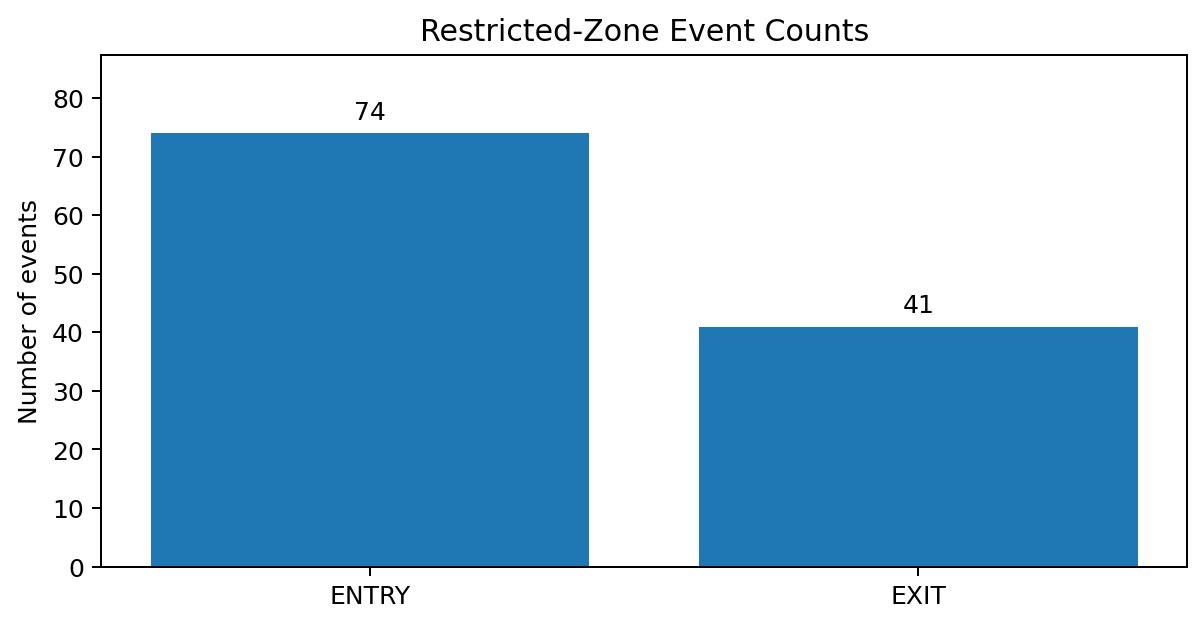
\includegraphics[width=0.78\textwidth]{figures/event_counts.png}
\caption{Observed ENTRY and EXIT event counts in the supplied runtime CSV log.}
\label{fig:eventcounts}
\end{figure}

\begin{table}[H]
\centering
\caption{Summary of the supplied runtime event CSV.}
\label{tab:event_summary}
\begin{tabular}{lr}
\toprule
Metric & Observed value\\
\midrule
Total events & 115\\
ENTRY events & 74\\
EXIT events & 41\\
Unique track IDs & 62\\
First timestamp & 00:00:00.000\\
Last timestamp & 00:00:15.000\\
First frame & 0\\
Last frame & 450\\
\bottomrule
\end{tabular}
\end{table}

For traceability, the first twelve records of the supplied log are reproduced below. The complete CSV is retained in the report evidence folder.

\begin{longtable}{llll}
\caption{First twelve records from the supplied runtime event log.}\label{tab:event_sample}\\
\toprule
Timestamp & Frame & Track ID & Status\\
\midrule
\endfirsthead
\toprule
Timestamp & Frame & Track ID & Status\\
\midrule
\endhead
00:00:00.000 & 0 & 4 & ENTRY\\
00:00:00.000 & 0 & 6 & ENTRY\\
00:00:00.000 & 0 & 9 & ENTRY\\
00:00:00.133 & 4 & 10 & ENTRY\\
00:00:00.567 & 17 & 7 & ENTRY\\
00:00:00.600 & 18 & 7 & EXIT\\
00:00:00.967 & 29 & 14 & ENTRY\\
00:00:01.000 & 30 & 14 & EXIT\\
00:00:01.200 & 36 & 15 & ENTRY\\
00:00:01.533 & 46 & 16 & ENTRY\\
00:00:01.767 & 53 & 17 & ENTRY\\
00:00:01.800 & 54 & 17 & EXIT\\
\bottomrule
\end{longtable}

\chapter{Testing and Evaluation}
\section{Automated Testing}
The final development snapshot contains tests for preprocessing, tracking, motion processing, semantic labeling, YOLO adapter behavior, drawing/overlay logic, and restricted-zone events. The authoring environment executed the suite with:
\[
\textbf{31 passed}
\]
within approximately 0.09 seconds. This is a software-test result for the development snapshot; it is not a video-performance benchmark.

\section{Evaluation Methodology}
The runtime screenshots and event CSV described in Chapter 9 provide qualitative and traceability evidence from an actual local run. The evaluation plan compares four scheduler configurations: every-frame YOLO, fixed frame skipping, adaptive skipping, and adaptive skipping with velocity smoothing plus refresh cooldown. All configurations should use the same input video and machine settings. Runtime, output FPS, YOLO call count, tracking statistics, flow magnitude, and zone-event quality are recorded in \code{evaluation/results\_template.csv}.

\section{Performance Metrics}
For a labeled evaluation clip, event performance is reported using:
\[
Precision = \frac{TP}{TP+FP}, \qquad Recall = \frac{TP}{TP+FN},
\]
\[
F1 = 2\frac{Precision\times Recall}{Precision+Recall}.
\]
Entry and exit metrics should be reported separately when labels permit it. A tolerance window of plus or minus three frames is recommended for matching predicted and manually annotated transitions.

\section{Benchmark Status}
No final video benchmark values are inserted in this report because the target evaluation machine, final clip, and runtime conditions must be measured by the project author. The package includes a benchmark plan and CSV template so those measurements can be added without changing the report structure. This avoids presenting unmeasured values as project evidence.

\chapter{Discussion}
\section{Strengths of the Design}
\begin{itemize}[leftmargin=*]
  \item The detector, tracker, event engine, and UI are modular and independently testable.
  \item The same track IDs are preserved across detector refreshes.
  \item Zone state is represented explicitly, enabling ENTRY and EXIT rather than repeated threshold alerts.
  \item Adaptive scheduling reduces semantic detector calls in calm scenes while prioritizing fast motion and restricted-zone activity.
  \item Dashboard and CSV output make system behavior inspectable instead of hiding results inside a video file.
\end{itemize}

\section{Limitations}
\begin{itemize}[leftmargin=*]
  \item The centroid tracker is a lightweight academic tracker and is not equivalent to more sophisticated multi-object tracking methods.
  \item YOLO predictions depend on scene quality, occlusion, lighting, model size, and confidence threshold.
  \item The adaptive velocity thresholds are expressed in pixels per frame and are therefore scene/camera dependent.
  \item The current project scope does not include camera calibration, stereo depth, 3-D reconstruction, or face recognition.
  \item No claim of production-grade surveillance reliability is made.
\end{itemize}

\section{Ethical and Privacy Considerations}
Video surveillance can contain personal information. For academic demonstrations, use consented or properly licensed footage. Keep stored data to the minimum needed for evaluation, avoid unnecessary identity inference, protect exported videos and event logs, and comply with institutional and applicable legal requirements. IntrudeAware is designed here as an academic video-analysis prototype rather than an autonomous decision-making system.

\chapter{Challenges Faced and How They Were Addressed}
\begin{longtable}{p{0.27\textwidth}p{0.62\textwidth}}
\toprule
Challenge & Resolution\\
\midrule
Python test imports & Added a repository-level \code{pytest.ini} with the project root on the Python path.\\
Optical-flow scalar conversion issue & Reshaped valid Lucas-Kanade point arrays before scalar extraction.\\
Browser video playback & Added a browser-compatible transcoding path using imageio-ffmpeg and H.264-compatible output.\\
Repeated zone events & Added explicit zone state, missing-frame grace, and re-entry cooldown.\\
Semantic labels & Replaced heuristic vehicle labeling with a YOLO semantic detector while keeping the existing tracker/event APIs.\\
YOLO compute cost & Added frame skipping, adaptive scheduling, velocity smoothing, and refresh cooldown.\\
Pylance overload warning & Passed an explicitly allocated output array to \code{calcOpticalFlowPyrLK}.\\
\bottomrule
\end{longtable}

\chapter{Future Enhancements}
\begin{enumerate}[leftmargin=*]
  \item Calibrate perspective and map pixel velocities into scene-relative measurements.
  \item Evaluate stronger trackers such as ByteTrack or BoT-SORT while preserving the same event API.
  \item Add line-crossing analytics and dwell-time statistics.
  \item Add a labeled evaluation dataset and report precision, recall, and F1 for semantic detection and events.
  \item Compare CPU, CUDA, and export formats such as ONNX/TensorRT on the same hardware.
  \item Add a persistent event database if long-term logging becomes necessary.
  \item Extend the system toward multi-camera views, depth estimation, or other topics from the CSE3010 syllabus in a separate research module.
\end{enumerate}

\chapter{VITyarthi Requirement Traceability}
The VITyarthi guide requires functional and non-functional requirements, architectural and workflow diagrams, UML/design artifacts, dataset/model-evaluation documentation where applicable, a GitHub repository, and a detailed report \cite{vityarthi_guide}. Table~\ref{tab:traceability} maps these requirements to the project package.

\begin{longtable}{p{0.35\textwidth}p{0.53\textwidth}}
\caption{Traceability of submission requirements.}\label{tab:traceability}\\
\toprule
Requirement & Evidence in this package\\
\midrule
Three or more major functional modules & Preprocessing, YOLO detection, tracking, motion, events, dashboard\\
Four or more non-functional requirements & Performance, usability, reliability, maintainability, scalability, logging\\
Architecture and workflow & Figures~\ref{fig:architecture} and \ref{fig:workflow}\\
UML/design diagrams & Figures~\ref{fig:usecase}, \ref{fig:sequence}, and \ref{fig:class}\\
Testing & \code{tests/} plus automated-test summary in Chapter 10\\
Model/dataset evaluation & \code{evaluation/benchmark\_plan.md} and \code{evaluation/results\_template.csv}\\
Repository documentation & \code{README.md} and \code{statement.md}\\
Final report & This PDF and its LaTeX source\\
\bottomrule
\end{longtable}

\chapter{Conclusion}
IntrudeAware integrates multiple CSE3010 computer-vision concepts into a single practical application. The final system combines preprocessing, YOLO semantic detection, persistent tracking, optical flow, restricted-zone state transitions, adaptive inference scheduling, and interactive reporting. The architecture deliberately keeps semantic detection decoupled from the tracker and event engine, enabling performance-oriented scheduling without changing the downstream behavior.

The implementation is sufficiently modular for continued development and sufficiently documented for academic evaluation. The remaining project-author task is to run the supplied evaluation protocol on the final target machine and fixed video, record the measured results in the evaluation CSV, replace the report placeholders with student information, and publish the repository to GitHub.

\appendix
\chapter{Installation and Usage}
\section{Windows PowerShell}
\begin{lstlisting}[language=bash]
cd IntrudeAware
python -m venv .venv
.\\.venv\\Scripts\\Activate.ps1
pip install -r requirements.txt
python -m pytest -q
streamlit run app.py
\end{lstlisting}

\section{Recommended first-run settings}
\begin{itemize}[leftmargin=*]
  \item YOLO model: Nano (\code{yolo26n.pt})
  \item Device: CPU unless CUDA is available and desired
  \item Confidence: 0.35
  \item Maximum frame skip: 3
  \item Adaptive frame skipping: enabled
  \item Velocity smoothing alpha: 0.35
  \item Refresh cooldown: 2 frames
\end{itemize}

\chapter{Selected Source Files}
\section{Core dependencies}
\begin{lstlisting}
streamlit>=1.38,<2.0
opencv-python>=4.10,<5.0
numpy>=1.26,<3.0
pandas>=2.2,<4.0
matplotlib>=3.9,<4.0
pytest>=8.0,<9.0
imageio-ffmpeg>=0.5,<1.0
ultralytics>=8.3,<9.0
\end{lstlisting}

\section{Project Configuration}
The default YOLO configuration is represented by the following values:
\begin{lstlisting}[language=Python]
YOLOConfig(
    model="yolo26n.pt",
    confidence=0.35,
    image_size=640,
    device="cpu",
    frame_skip=3,
    adaptive_frame_skip=True,
    velocity_smoothing_alpha=0.35,
    refresh_cooldown_frames=2,
)
\end{lstlisting}

\chapter{References}
\begin{thebibliography}{9}
\bibitem{cse3010_syllabus} VIT University / School of Computing, \emph{CSE3010 Computer Vision Course Learning Plan}, 2020.
\bibitem{vityarthi_guide} VITyarthi, \emph{Build Your Own Project - General Project Instructions and Submission Guidelines}, supplied project guide.
\bibitem{szeliskiref} R. Szeliski, \emph{Computer Vision: Algorithms and Applications}, Springer, 2011.
\bibitem{hartleyref} R. Hartley and A. Zisserman, \emph{Multiple View Geometry in Computer Vision}, 2nd ed., Cambridge University Press, 2004.
\bibitem{ultralytics_yolo26} Ultralytics, \emph{Ultralytics YOLO26 Documentation}, 2026. \url{https://docs.ultralytics.com/models/yolo26}
\bibitem{opencvref} OpenCV, \emph{OpenCV Documentation}, 2026. \url{https://docs.opencv.org/}
\end{thebibliography}

\end{document}
